\Chapter{Útvonalkereső heurisztikák}

\Section{Probléma felírása}

% útvonaltervezés, optimalizáció, keresési eljárások
Az alapvető cél, amit el szeretnénk érni, az találni egy optimális útvonalat, amely az akadályokat kikerülve eljuttatja a járművet valahová. Több megoldást is be fogok mutatni, az egyszerűbbektől a bonyolultabbakig. A kísérletek eredményei is láthatóak lesznek, melyek véletlenszerűen generált útvonalakat fognak ábrázolni bizonyos paraméterek alapján. Ezek után konkrét algoritmusokat fogok definiálni és bemutatni, melyek már tényleges optimumot adnak és adott kezdőpontból adott végpontba juttatják a járművet. 


\Section{Véletlen bolyongás}

Az első és legegyszerűbb (bár kevésbé hatékony) megoldás a véletlenszerű útvonalak generálása. Ennek lényege, hogy minél több útvonal közül ki tudja választani a gép azt, ami a legközelebb esik az elérni kívánt koordinátához vagyis a célhoz és nem ütközik egy akadályba sem, amelyek pozícióit mi határozzuk meg. Ezek definiálása a későbbiekben fog megtörténni.\\ 

\subsection{Útvonal generálás módszerei}

A véletlen útvonalakat jelen esetben úgy kell elképzelni, hogy a jármű kap bizonyos adatokat, hogy milyen szögben forduljon el adott időpillanatban. Tehát a kanyarodási szögek lesznek véletlenek és ezekből számítódnak majd az útvonalak. Elfordulás generálási módszer alapján figyelembe vehetünk két esetet:\\
\phantom{len}- abszolút elfordulás\\ 
\phantom{len}- relatív elfordulás\\
Abszolút elfordulás alatt azt értjük, hogy a generált szög lesz a jármű kanyarodási szöge, mindegy mi volt az előző elfordulás értéke. Relatív esetben pedig a generált szög mindig az előzőhöz adódik hozzá. Mindkét esetre láthatunk majd példákat, melyik megoldással milyen végpontokba juthatunk el vagy milyen útvonalakat kaphatunk. Be is mutatnám ezen paraméterek alapján az útvonal meghatározását és megvizsgálhatjuk az elérhető pontok eloszlását valamint valószínűségét.\\\\
Python program a relatív elfordulásos esetre:

\begin{python}
import math
from matplotlib import pyplot as plt
import random
\end{python}
Szükséges importok.

\begin{python}
def generate_random_angles_relative(number_of_turns):
        rel_angles = []
        angles = []
        for i in range(number_of_turns):
            angle = random.randint(-35, 35)
            angles.append(angle)
        for a in range(len(angles)):
            if a == 0:
                rel_angles.append(angles[0])
            else:
                rel_angles.append(angles[a])
                rel_angles[a] = angles[a] + rel_angles[a-1]
        return rel_angles
\end{python}
A függvény paraméterként az elfordulások számát várja. A belsejében pedig annyi random számot generál, amennyi ez az érték. A random szám alapértelmezett esetben -35 és +35, melyet az $angle$ változóba tárolok, majd hozzáadom őket egyesével egy listához. A maximum kanyarodási szög értéke sokmindentől függhet. A példában lévő szám egy teljesen átlagos elfordulási szögnek vehető egy személyautót tekintve. Szükséges lesz még egy for ciklus, amiben a generált szögeken végigmegyünk, majd az aktuális értékhez hozzáadjuk az előzőt (kivéve az elsőhöz). Így megkapjuk a kívánt értékeket. 

\begin{python}
rand_angles_rel = generate_random_angles_relative(30)
\end{python}
A függvény visszatérési értékét eltároljuk egy változóba. Paraméterként megadjuk, hogy hány kanyarodás történjen.

\begin{python}
def calc_path(pos_x, pos_y, steering_angles):
        path = []
        for deg in steering_angles:
            pos_x = pos_x + math.cos(math.radians(deg))
            pos_y = pos_y + math.sin(math.radians(deg))
            path.append((pos_x, pos_y))
        return path
\end{python}
A $calc\_path$ függvénnyel pedig az útvonalat tudjuk kiszámolni. Itt a kezdőpozíció $ x $ és $ y $ koordinátáit adhatjuk meg paraméterként, valamint a generált elfordulási szögeket, melyet a $rand\_angles\_rel$ változóban tárolunk. Itt is for ciklussal kell kiszámolnunk minden szögnél az adott pozíciót. Az aktuális pozícióhoz mindig hozzáadjuk az előzőt és az adott szög szinuszát és koszinuszát (annak függvényében, hogy $ x $ vagy $ y $ pozícióról van szó). 

\begin{python}
random_relative_path = calc_path(0, 0, rand_angles_rel)

x_random_relative = list(zip(*random_relative_path))[0]
y_random_relative = list(zip(*random_relative_path))[1]
\end{python}
A függvény meghívása, majd formázása a kirajzoláshoz. $ (x, y) $ alakról (tuple típusú változó) kell lebontani egy listába külön az $ x $ és külön az $ y $ értékeket. Ezt a $ zip $ funkcióval és a $ * $ operátor segítségével tehetjük meg.\\

\begin{python}
plt.plot(x_random_relative, y_random_relative, 'black')
plt.xlabel("x coordinates")
plt.ylabel("y coordinates")
plt.savefig('relative_example_path.png')
plt.show()
\end{python}
Ha pedig az eredményre vagyunk kíváncsiak, a $ matplotlib.pyplot $ könyvtár  $ plot() $ függvényét hívhatjuk meg, amely az x és y koordinátákat várja paraméternek és kirajzolja a grafikont. Ezzel kaptunk is egy példa útvonalat:

\begin{figure}[h!]
\centering
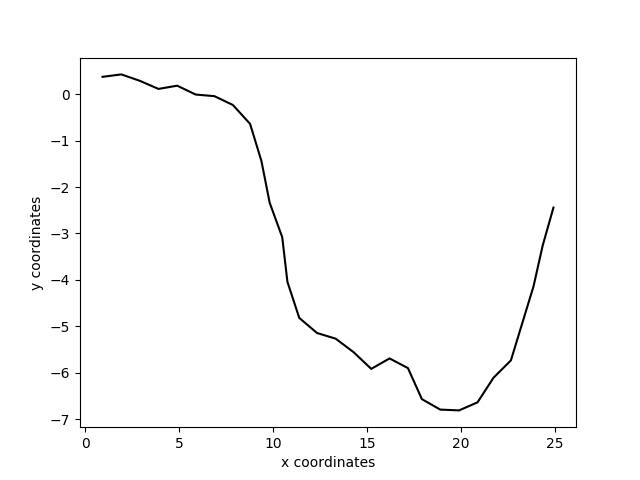
\includegraphics[scale=0.75]{images/relative_example_path.png}
\caption{Relatív random példa útvonal}
\label{fig:relative_path}
\end{figure}

Python program az abszolút elfordulásos esetre:

\begin{python}
def generate_random_angles_absolute(number_of_turns):
    random_angles = []
    for i in range(number_of_turns):
        angle = random.randint(-35, 35)
        random_angles.append(angle)
    return random_angles
    
def calc_path(pos_x, pos_y, steering_angles):
    path = []
    for deg in steering_angles:
        pos_x = pos_x + math.cos(math.radians(deg))
        pos_y = pos_y + math.sin(math.radians(deg))
        path.append((pos_x, pos_y))
    return path
    
rand_angles_absolute = generate_random_angles_absolute(30)

random_absolute_path = calc_path(0, 0, rand_angles_absolute)

x_random_absolute = list(zip(*random_absolute_path))[0]
y_random_absolute = list(zip(*random_absolute_path))[1]

plt.plot(x_random_absolute, y_random_absolute, 'blue')
plt.xlabel("x coordinates")
plt.ylabel("y coordinates")
plt.savefig('absolute_example_path.png')
plt.show()
\end{python}
Itt a generálás módja jóval egyszerűbb, ténylegesen csak egy random szám, amit nem ad hozzá az előző értékhez. Ez esetben az eredmény kevésbé reális, szinte minden útvonalban lesznek olyan szakaszok, ahol jelentős kólönbség van az előző és az aktuális szög között, így nagyobb törés figyelhető meg a vonalon.

\begin{figure}[h!]
\centering
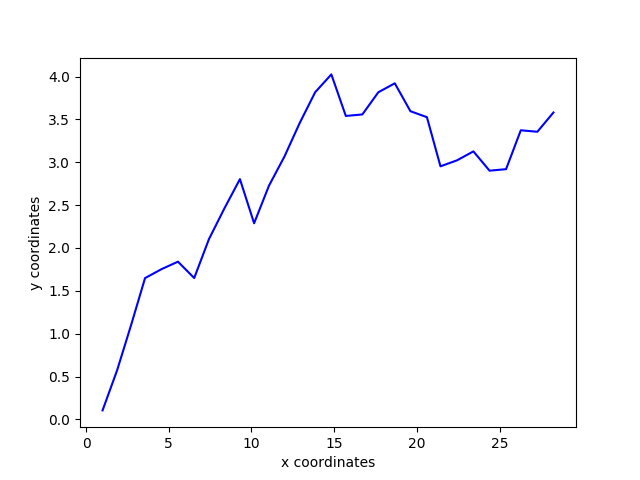
\includegraphics[scale=0.75]{images/absolute_example_path.png}
\caption{Abszolút random példa útvonal}
\label{fig:absolute_path}
\end{figure}

\newpage
\subsection{Végpontok eloszlása, valószínűségi grafikonok}

Ebben az alpontban megvizsgáljuk, hogy különböző paraméterek esetén melyik pozícióba hány alkalommal, illetve milyen valószínűsággel juthatunk el. Legyen az alapértelmezett érték 1000 db generálás. Tehát ennyi útvonalat fognak a függvények meghatározni és kigyűjtöm a végpontok $ x $ és $ y $ koordinátáit 2 külön listába. Ez alapján meghatározható az értékek eloszlása.\\\\
Első esetben az elfordulások száma 30, kanyarodási szög -35$^{\circ}$, +35$^{\circ}$ közötti, generálás módszere relatív, a kezdőpozíció az origó (0, 0).\\

A \ref{fig:relative_x_endpos}. ábrán megfigyelhetjük az adott végpozíciók $ x $ koordinátáinak előfordulását. Az x tengelyen az $ x $ koordináták láthatók, az y tengelyen pedig hogy 1000-ből hányszor fordult elő. A diagramon exponenciális növekedés figyelhető meg, legtöbbször a 25-ös $ x $ koordinátába juthatunk el. Ezt többször is lefuttattam, mindegyiknél hasonló eredmény figyelhető meg, általában 23-27 közötti pontokat érhetünk el legtöbbször. Negatív értékek is megfigyelhetők, ilyenkor fordulatot vesz a jármű és ellenkező irányba halad.\\

A \ref{fig:relative_y_endpos}. ábrán is ugyanezeket az adatokat figyelhetjük meg, csak az y koordináták esetében. Itt a leggyakoribb értékek a -22 és a +19, de a -8, +8 értékek gyakorisága is hasonló. Itt már nagyobb véletlenszerűség látszódik.\\

A \ref{fig:relative_x_endpos_density}. és a \ref{fig:relative_y_endpos_density}. grafikonok az előzőek mintájára készült annyi különbséggel, hogy az y tengelyen valószínűségi érték látható.
\newpage 


\begin{figure}[h!]
\centering
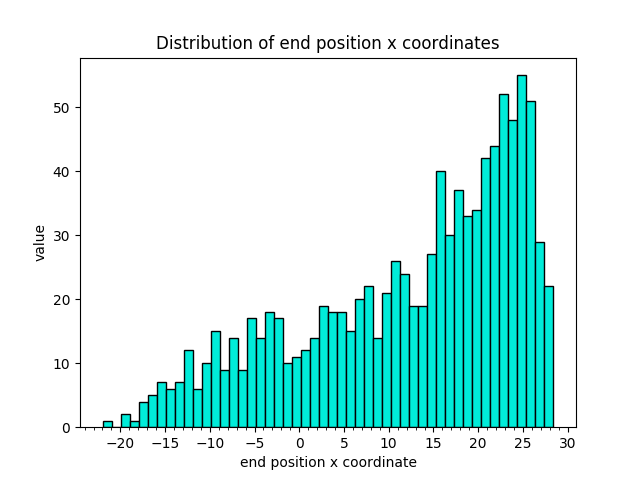
\includegraphics[scale=0.75]{images/relative_x_endpos.png}
\caption{Elérhető x koordináták eloszlása szám szerint}
\label{fig:relative_x_endpos}
\end{figure}

 

\begin{figure}[h!]
\centering
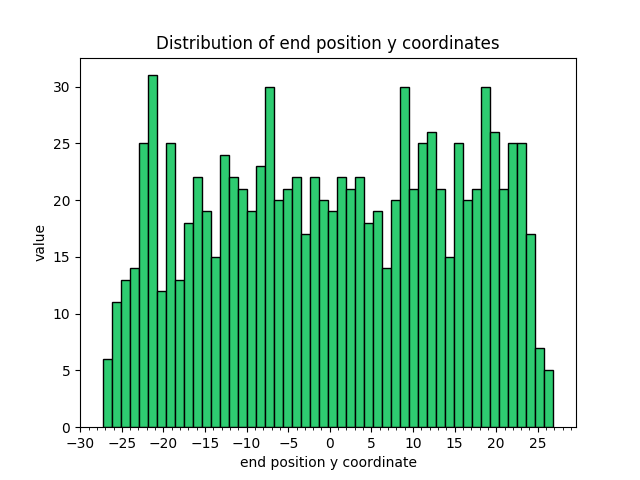
\includegraphics[scale=0.75]{images/relative_y_endpos.png}
\caption{Elérhető y koordináták eloszlása szám szerint}
\label{fig:relative_y_endpos}
\end{figure}

\begin{figure}[h!]
\centering
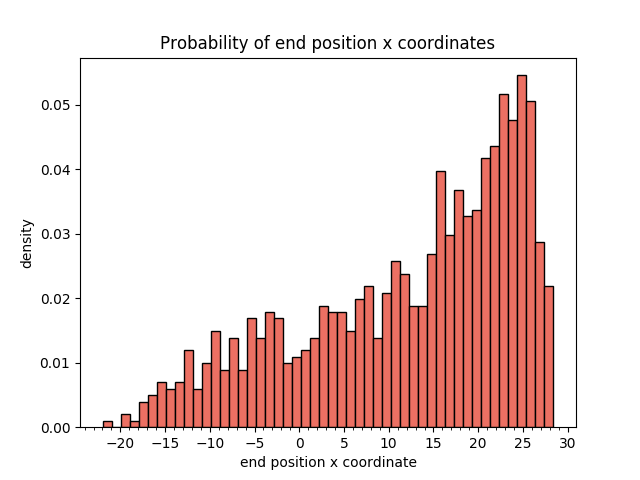
\includegraphics[scale=0.75]{images/relative_x_endpos_density.png}
\caption{Elérhető x koordináták valószínűsége}
\label{fig:relative_x_endpos_density}
\end{figure}

\begin{figure}[h!]
\centering
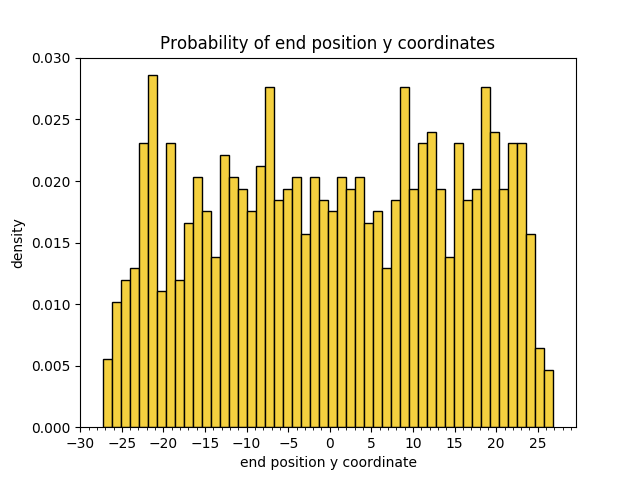
\includegraphics[scale=0.75]{images/relative_y_endpos_density.png}
\caption{Elérhető y koordináták valószínűsége}
\label{fig:relative_y_endpos_density}
\end{figure}

\newpage

\Section{Gépi tanítás a probléma inverzével}

% TODO: Véletlenszerű útvonalakhoz (mint jó megoldásokhoz) generálni akadályokat, és úgy tekinteni, hogy ez az algoritmus be- és kimenetére egy-egy példát jelent.
